\documentclass[a4paper]{article}
\usepackage[utf8]{inputenc}
\usepackage[spanish, es-tabla, es-noshorthands]{babel}
\usepackage[table,xcdraw]{xcolor}
\usepackage[a4paper, footnotesep = 1cm, width=20cm, top=2.5cm, height=25cm, textwidth=18cm, textheight=25cm]{geometry}
%\geometry{showframe}

\usepackage{tikz}
\usepackage{amsmath}
\usepackage{amsfonts}
\usepackage{amssymb}
\usepackage{float}
\usepackage{graphicx}
\usepackage{caption}
\usepackage{subcaption}
\usepackage{multicol}
\usepackage{multirow}
\setlength{\doublerulesep}{\arrayrulewidth}
\usepackage{booktabs}

\usepackage{hyperref}
\hypersetup{
    colorlinks=true,
    linkcolor=blue,
    filecolor=magenta,      
    urlcolor=blue,
    citecolor=blue,    
}

\newcommand{\quotes}[1]{``#1''}
\usepackage{array}
\newcolumntype{C}[1]{>{\centering\let\newline\\\arraybackslash\hspace{0pt}}m{#1}}
\usepackage[american]{circuitikz}
\usetikzlibrary{calc}
\usepackage{fancyhdr}
\usepackage{units} 

\graphicspath{{../Ejercicio-1/}{../Ejercicio-2/}{../Ejercicio-3/}{../Ejercicio-4/}}

\pagestyle{fancy}
\fancyhf{}
\lhead{22.01 Teoría de Circuitos}
\rhead{Mechoulam, Lambertucci, Rodriguez Turco, Londero, Galdeman}
\rfoot{\centering \thepage}

\begin{document}

Las hipótesis realizadas en los siguientes análisis del circuito base se comprobarán más adelante a la hora de realizar las simulaciones y el subsiguiente prototipeado.

\subsection{Análisis Cualitativo del Circuito Base}

\subsubsection{Etapa de Alimentación}

La alimentación del circuito es una fuente no partida de $9V$. Se observa que el capacitor electrolítico $C_5$ se encuentra justo a la salida de la fuente de alimentación. Este capacitor no solo filtrará cualquier ruido que haya montado sobre la continua u ocasional \textit{ripple} que pueda hallarse, ya que por su conexión a tierra, cualquier tensión no contante encontrará un camino de baja impedancia hacia masa, sino también que funcionará como capacitor de desacople para el amplificador operacional, siempre y cuando este esté posicionado físicamente lo más cerca posible del integrado, para eliminar inductancias parásitas que no puedan permitir un pico de consumo de corriente.

\begin{figure}[H]
	\centering
	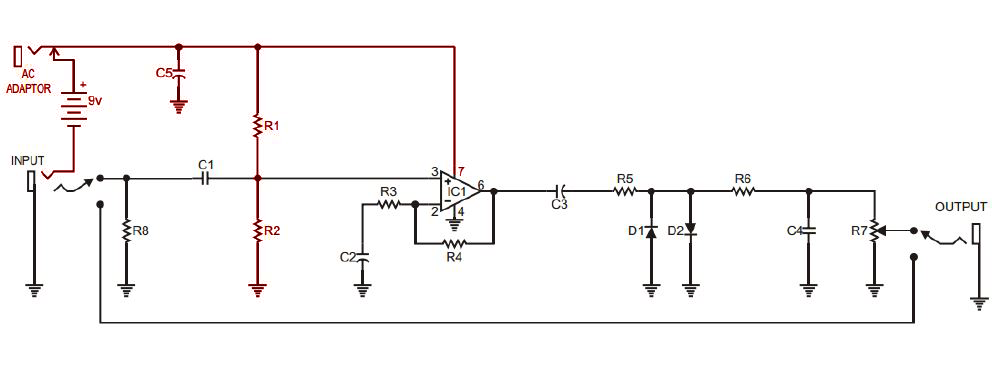
\includegraphics[width=1\textwidth, trim={0 0 0 0}, clip]{Ejercicio5/Imagenes/Circuito_base/circuito_base_alimentacion.png}
	\caption{Alimentación del circuito base.}
	\label{fig:circuito_base_alimentacion}
\end{figure}

Luego pueden verse dos resistencias $R_1$ y $R_2$, donde $R_1$ está conectada a la señal de entrada y $R_2$ está conectada a la resistencia anterior y a tierra. Este par puede considerarse de manera aproximada como un divisor resistivo, ya que en el punto medio se ofrece gran impedancia por parte tanto del op-amp como por el capacitor $C_1$ (por ser tensión continua) lo que significa que la corriente que fluya por otro medio que no sea la resistencia $R_2$ será despreciable.
Este divisor resistivo monta a la señal de entrada sobre la tensión en el punto medio. Es en este punto donde se soluciona el problema de tener una sola fuente no partida ya que, si se cumple que $R_1=R_2$, la señal de entrada quedará levantada $4.5V$, por lo que se podría alimentar al op-amp solo de manera positiva, llevando a tierra la alimentación negativa.\\

Por último, se llevan los $9V$ de la fuente de alimentación a la entrada de alimentación positiva del op-amp.


\subsubsection{Etapa de Pre-amplificación}

\begin{figure}[H]
	\centering
	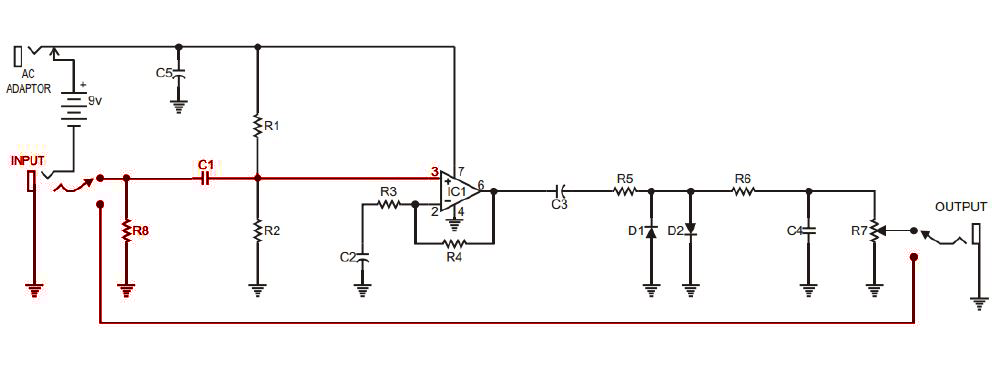
\includegraphics[width=1\textwidth, trim={0 0 0 0}, clip]{Ejercicio5/Imagenes/Circuito_base/circuito_base_preamplificacion.png}
	\caption{Etapa de pre-amplificación del circuito base.}
	\label{fig:circuito_base_preamplificacion}
\end{figure}

Justo luego de la entrada se encuentra la resistencia $R_8$. En el modo de operación normal del circuito con la guitarra conectada, se polariza el capacitor $C_1$ debido a la continua provista por la alimentación. La finalidad de esta resistencia es de mantener polarizado al capacitor cuando se desconecta el efecto del circuito, es decir, cuando se utiliza la llave de bypass. Si este capacitor se descarga por pérdidas parásitas antes de volver a conectar el efecto, se da a lugar el famoso ruido de 'pop' que puede escucharse.

Para explicar este efecto con mayor detalle, imaginar que no se tiene la resistencia $R_8$ y está conectada la guitarra al circuito. Cuando la 'placa' de la derecha del capacitor $C_1$ está conectada a una tensión de $4,5V$, la 'placa' de la izquierda permanecerá polarizada con $0V$ ya que esta está conectada al pickup de la guitarra que a su vez está conectado a tierra. Al momento de utilizar la llave de bypass, como el capacitor no es ideal, este tendrá pequeñas pérdidas que harán que la tensión con la que está cargado el capacitor disminuya, ya que la 'placa' izquierda no estará conectada a nada. Cuando se decida volver a utilizar la llave de bypass, es decir, utilizar el efecto del circuito, se volverá a cargar al capacitor con la tensión de bias proporcionada por el divisor resistivo, necesitando un rápido flujo de carga, es decir, corriente. Esta descarga de corriente será enviada al parlante, el cual producirá un sonido distintivo. Si se coloca la resistencia $R_8$, la 'placa' izquierda del capacitor permanece siempre a $0V$ y por ende no tomará a lugar el efecto dicho.

El capacitor $C_1$, como ya dicho antes, ofrece gran impedancia a la tensión continua de la alimentación para proteger a la entrada. De otra manera, la señal continua ingresaría por la entrada.
Lo que se obtiene posterior al capacitor será la señal de entrada levantada tantos voltios como proporcionen el punto medio del divisor resistivo.\\

Se contempla además que el circuito base nos permite tener una opción de realizar un bypass total al circuito mediante el uso de una llave.

\subsubsection{Etapa de Amplificación}

El operacional se encuentra realimentado negativamente con una configuración no inversora. El hecho de que la alimentación positiva sea de $9V$ y la negativa de $0V$ significa que la señal de salida del operacional podrá tener un valor mínimo de a lo sumo $0V$ y un valor máximo de a lo sumo $9V$ (dependiendo del operacional utilizado). Como la señal de entrada estará montada sobre una continua, esto no será un problema.

\begin{figure}[H]
	\centering
	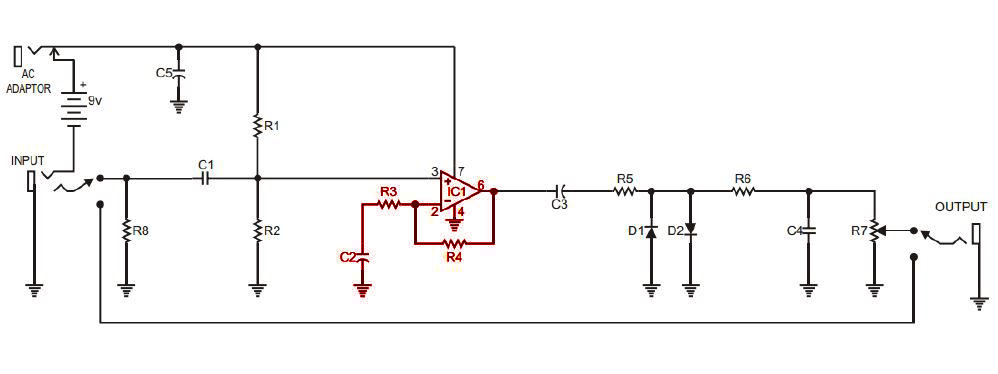
\includegraphics[width=1\textwidth, trim={0 0 0 0}, clip]{Ejercicio5/Imagenes/Circuito_base/circuito_base_amplificacion.png}
	\caption{Etapa de amplificación del circuito base.}
	\label{fig:circuito_base_amplificacion}
\end{figure}

Analizando el lazo del op-amp, se puede observar que la ganancia dependerá de la frecuencia.
Esto puede contemplarse ya que para bajas frecuencias el capacitor actúa con gran impedancia, por lo que el operacional amplifica menos. Para las frecuencias altas el operacional amplificará idealmente cada vez más la señal. Sin embargo, mas importante es que este capacitor impide que el operacional amplifique la continua sobre la cual está montada la señal, ya que en este caso el capacitor se comporta como un circuito abierto. Esto hace que el operacional funcione como un seguidor de tensión, trabajando para fijar la continua de la salida en el mismo valor que la de la referencia. Se observa como es aquí, en el lazo de realimentación, donde se podría controlar la amplificacion de las distintas frecuencias por separado, si se desease por ejemplo utilizar un potenciómetro más adelante para tener un control de tono.

\subsubsection{Etapa de Ecualización}

A la salida del operacional se encuentra el capacitor $C_3$. Este capacitor se utiliza para remover la continua sobre la cual estaba montada la señal de entrada.

\begin{figure}[H]
	\centering
	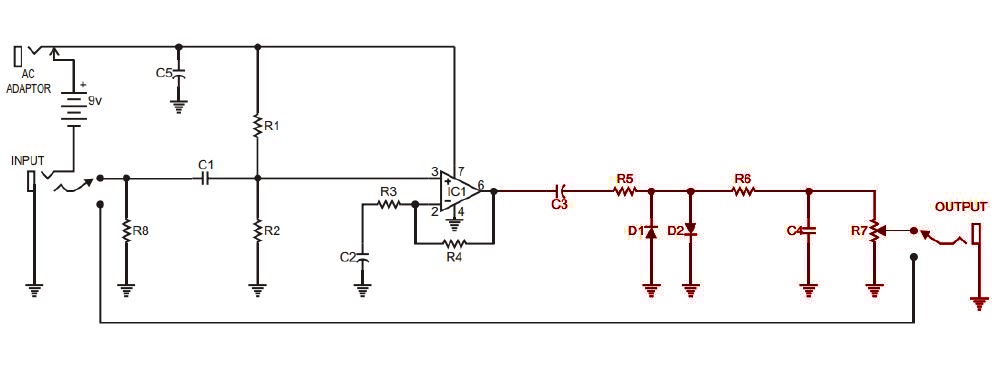
\includegraphics[width=1\textwidth, trim={0 0 0 0}, clip]{Ejercicio5/Imagenes/Circuito_base/circuito_base_ecualizacion.png}
	\caption{Etapa de ecualización del circuito base.}
	\label{fig:circuito_base_ecualizacion}
\end{figure}

Luego, se encuentra en el circuito una resistencia en serie con un par de diodos en paralelo con polaridad invertida. Estos diodos fijarían la tensión de la señal en $V_{d_{on}}$ tanto para el semi-ciclo positivo como para el negativo, deformando la señal generando un efecto de \textit{clipping}. Esto se aprecia como una gran distorsión a la hora de conectar una guitarra y escuchar la salida. La resistencia $R_5$ limitará la corriente que atraviesa los diodos.  \\

Seguido de los diodos se puede encontrar un pequeño circuito R-C. Este circuito estaría posicionando un polo en la respuesta en frecuencia, atenuando las frecuencias altas. 

Finalmente antes de la salida se encuentra un potenciómetro, el cual se presume que se utiliza como control de volumen de salida.

\subsubsection{Corriente de Bias y Tensión de Offset}
La corriente de bias como la tensión de offset pueden ocasionar que la salida del operacional sea distinta de cero aportando una componente de continua aunque la entrada sea nula. En esta aplicación, tanto la corriente de bias como la tensión de offset no son un problema, ya que:
\begin{itemize}
\item Se le proporciona a la entrada gracias a la fuente de alimentación la suficiente corriente al operacional para la correcta polarización de todos los elementos que puedan hallarse dentro de este, sin preocupación alguna por la muy pequeña corriente que pueden suministrar los pickups de una guitarra.
\item Gracias a los capacitores de acople situados en el circuito la componente de continua de la señal de salida del operacional es removida completamente.
\item Un muy pequeño desbalanceo en la tensión de bias de la señal de entrada al operacional produciría en el peor de los casos una saturación asimétrica que contribuiría a la distorsión alineal total del circuito.
\end{itemize} 

\subsection{Análisis Cuantitativo del Circuito Base}

Tanto el análisis cuantitativo como el subsiguiente diseño de un nuevo circuito propuesto se harán a partir de lo estudiado en tanto diversas fuentes de internet, como en el libro 'Diseño de Amplificadores Operacionales y Circuitos Integrados Analógicos' de Sergio Franco.

Además, se decidió, para presentar lo realizado de la forma más clara, primero realizar un análisis teórico-analítico del circuito base para luego presentar sólamente los cambios propuestos.

\subsubsection{Componentes}

\textbf{$R_8$:}
Esta resistencia debe tener un valor alto para no tener perdida substancial de corriente provista por las bobinas de los pickups y no limitar la impedancia de entrada del circuito vista por la guitarra. \textbf{Además, se puede calcular el tiempo característico del RC (entre $R_8$ y $C_1$) que dirá cuánto tardará el capacitor en descargarse. Sin embargo, esto último no se tomará en cuenta y se utilizará una resistencia de $1M\Omega$, ya que por más que el tiempo característico sea muy lento, de un par de segundos inclusive, para esta aplicación se supone que el usuario no estará conectando y desconectando el efecto cada menos de 5 segundos.} \\

\textbf{$R_1$, $R_2$:} Se quiere montar a la señal de entrada sobre una continua de la mitad del valor que la de la alimentación, por esto, se decidió que $R_1=R_2$.

Se consideraron los siguientes puntos a la hora de elegir un valor para las resistencias:
\begin{itemize}
\item Que la corriente en stand-by no sea muy alta.
\item No limitar tanto la impedancia de entrada.
\end{itemize}
\textbf{Sin embargo, se puede demostrar que cuanto más grande sea el valor de los resistores usados, más grande será el ruido, por lo que el valor de estos resistores se sitúan en una situación de compromiso.}
El valor utilizado es de $R_1=R_2=100 \ k\Omega$.\\

\textbf{$C_1$:} Como este capacitor filtra la continua provista por la alimentación, se decidió utilizar un valor de $330 \ nF$ ya que se quiso que el efecto del filtro pasa-altos que se forma con las resistencias $R_1$ y $R_2$ se minimizara dentro de las frecuencias audibles ($20Hz-20kHz$).
Si sólamente se tiene en cuenta la componente alterna del circuito, la resistencia $R_1$ pasa a estar conectada a tierra, por lo que se forma el paralelo entre $R_1$ y $R_2$. Finalmente utilizando la técnica del divisor resistivo se tiene que

\begin{equation}
H(s) = \frac{(R_1//R_2)}{(R_1//R_2) + \frac{1}{SC_1}}
\end{equation}

\begin{equation}
H(s) = \frac{SC_1(R_1//R_2)}{SC_1(R_1//R_2) + 1}
\end{equation}

donde puede calcularse la capacitancia necesaria como
\begin{equation}
C_1=\frac{1}{2\pi (R_1//R_2) f_c} = \frac{1}{2\pi 50k\Omega 10Hz} = 318,3nF \approx 330nF
\end{equation}

Cabe notar que el error proporcionado por la aproximación a un valor comercial no trae gran problema, ya que la frecuencia de corte aunque se desplace de los $10Hz$ aún estarán lejos de la banda audible.

\textbf{$C_5$:} Este capacitor filtrará el ruido proveniente de la alimentación, minimizará el \textit{ripple}, y funcionará como capacitor de desacople para el operacional, por lo que se eligió un valor de $100\mu F$, relativamente alto para lograr tener con seguridad una continua fiable, mientras que también pueda filtrar ruido a lo largo de una gran banda de frecuencias, por más que este no sea el mayor de los problemas.

\textbf{$R_4, R_3, C_2$:} Como ya dicho en la sección de análisis cualitativo, la ganancia de la etapa de amplificación dependerá de la frecuencia, y no solo esto, sino también de la ganancia a lazo abierto del operacional.

\begin{equation}
	V_{o_{opamp}} = \frac{A_0 V_{i_{opamp}}}{1+A_0 \frac{R_3 + \frac{1}{SC_2}}{R_4 + R_3 + \frac{1}{SC_2}}}
\end{equation}

Sin embargo, si se cumple en la banda audible de frecuencias que

\begin{equation}
\left| A_o\frac{R_3 + \frac{1}{SC_2}}{R_4 + R_3 + \frac{1}{SC_2}} \right| \gg 1
\label{cond_1/b}
\end{equation}

se tiene que

\begin{equation}
V_{o_{opamp}} \approx V_{i_{opamp}}\left( 1 + \frac{R_4}{R_3 + \frac{1}{SC_2}}  \right)
\end{equation}

\begin{equation}
	V_{o_{opamp}} \approx V_{i_{opamp}}\left( 1 + \frac{SC_2R_4}{SC_2R_3 + 1}  \right)
\end{equation}

Se eligieron valores de $R_4=51R_3=1k$ para lograr una ganancia máxima en la etapa de amplificación de $34, 32 \ dB$.
\[20log_{10}(1+\frac{R_4}{R_3}) = 34,32 \ dB\]
El capacitor además de no dejar amplificar la continua adjudica cuánto son amplificados los graves. Se utilizó un valor de $330nF$ calculándose la capacidad analizando el filtro que se forma con $R_3$ teniendo un grado de libertad a la hora de darle forma al sonido que se quiere producir. \textbf{Preguntar sobre estabilidad, amplificacion de bajos}

\[ C_2 = \frac{1}{2\pi f_c R_3} = \frac{1}{2\pi 500Hz 1k\Omega} = 318,3nF \approx 330nF \]

Se puede ver que se sigue cumpliendo la condición (\ref{cond_1/b}) ya que

$$ \left| A_o\frac{R_3 + \frac{1}{SC_2}}{R_4 + R_3 + \frac{1}{SC_2}} \right|_{f=20Hz} \approx 0,421A_0 $$
$$ \left| A_o\frac{R_3 + \frac{1}{SC_2}}{R_4 + R_3 + \frac{1}{SC_2}} \right|_{f=20kHz} \approx 0,019A_0 $$

y la ganancia a lazo abierto suele tener un valor en el orden de $10^5 \ a \ 10^6 $.\\

\textbf{$C_3$:} Este capacitor está solamente para filtrar la continua de la salida del operacional pero como forma un pasa-altos con la impedancia equivalente de salida del circuito que aproximadamente es de $8k\Omega$, y no se quiere que afecte este capacitor al circuito, su valor será de $10\mu F$ lo que dejaría la frecuencia de corte en $\approx 2Hz$, realizando la misma cuenta que para $C_1$.\\

\textbf{$R_5, R_6$:} $R_5$ se sitúa para limitar la corriente de los diodos, y $R_6$ para limitar la corriente de descarga del capacitor. El fabricante indica que la corriente máxima de continua que soporta el diodo 1N4148 es de $300mA$. Como después del capacitor $C_3$ la tensión máxima que puede haber en el circuito es de $4,5V$ pico, o de $\approx 3,2V_{rms}$, \textbf{la resistencia mínima que debe colocarse es de $\approx 10\Omega$. Sin embargo, por más que se quiera una impedancia baja de salida del circuito, se seleccionó un valor de $6,8k\Omega$ para tener un gran margen de seguridad.} $R_6$ formará un filtro pasabajos con $C_4$, por lo que, con cierto grado libertad, se eligió un valor de $1k\Omega$.\\

\textbf{$C_4$:} Como este capacitor forma un pasa bajos con la resistencia $R_6$, se eligió un valor de $6,8nF$ de tal manera que su frecuencia de corte se encuentre aproximadamente en $f_c = 20kHz$.
\[ C_4 = \frac{1}{2\pi 20kHz 1,2k\Omega} = 6,63nF \approx 6,8nF\]
Nuevamente, se realizó una aproximación con mucho error, por la libertad de diseño sonoro que se posee a la hora de posicionar los polos en la trasferencia. Debido al error cometido, el polo estará situado con una frecuencia de corte de $$ f_c = \frac{1}{2\pi 1,2k\Omega 6,8nF} = 19,5kHz $$

\textbf{$R_7$:} Este resistor será un potenciómetro logarítmico de $10k\Omega$ si hay disponibilidad en el pañol. El tipo de potenciómetro será logarítmico ya que de esta manera se acopla mejor a la escucha humana.\\

\textbf{$LM308$:} Se eligió el amplificador operacional $LM308$ con una compensación de $33pF$ por las siguientes razones:

\begin{itemize}
\item Impedancia de entrada relativamente alta ($10M\Omega$ en el peor de los casos) comparada con la contribución del resto de los componentes de los circuitos. Esto permitirá que no se limite la impedancia de entrada posible a causa del amplificador operacional.
\item Capacidad de compensar el operacional, haciendo tanto el ancho de banda como el slew rate proporcionales a la inversa de la capacitancia de compensación utilizada.
\item Excepcionalmente baja slew rate, lo que contribuye al efecto alineal de distorsión de la señal.
\end{itemize}

\subsubsection{Impedancia de Entrada}

\textbf{Para un circuito con esta aplicación se quiere como ya dicho la mayor impedancia de entrada posible para no perder agudos o armónicos.}
La impedancia de entrada del circuito base puede calcularse considerando solamente la señal alterna que recorre el circuito. Al hacer esto, se puede observar que la resistencia $R_1$ estará conectada a tierra, por lo que la impedancia de entrada será
\[Z_{in} = (R8//(R1//R2))//Z_{in_{opamp}} = (1M\Omega // 255k\Omega)//10M\Omega \approx 199k\Omega\]

\subsubsection{Impedancia de Salida}

\textbf{La impedancia de salida se quiere mantener lo más baja posible.}
Si se desprecia el potenciómetro a la salida para controlar el volúmen, la impedancia de salida del circuito base puede calcularse como
\[ Z_{out} = Z_{out_{opamp}} + 6k8\Omega + 1,2k\Omega \approx 8k\Omega \]

\subsection{Simulación del Circuito Base}

Se realizaron tres tipos de simulaciones diferentes para visualizar el funcionamiento del circuito.

\begin{figure}[H]
	\centering
	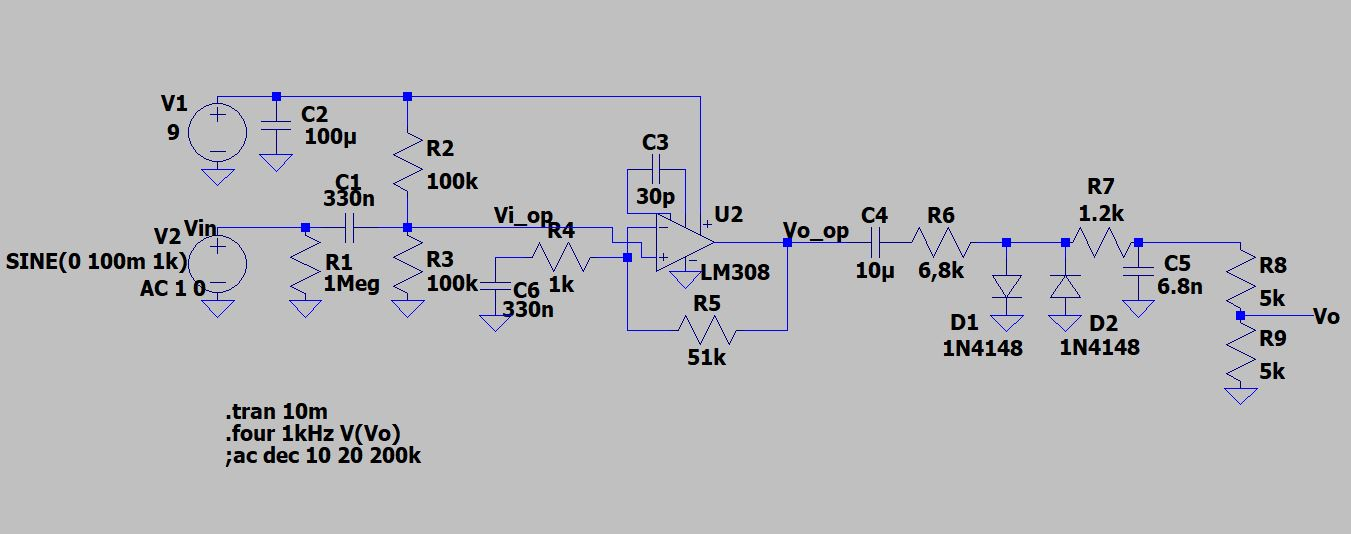
\includegraphics[width=1\textwidth, trim={0 0 0 0}, clip]{Ejercicio5/Imagenes/Circuito_base/Sim/sim_base.JPG}
	\caption{Set-up para los tres tipos de simulaciones distintas del circuito. Las dos resistencias del final emulaban un potenciómetro. Transitorio, AC-Sweep y análisis de Fourier.}
	\label{fig:sim_base}
\end{figure}

\subsubsection{Análisis de Señal, Transitorio}

Para simular el transitorio y poder observar la señal de entrada, se eligió una frecuencia de $1kHz$ y una amplitud de $100mV$ emulando una guitarra.
Primero se analizó el accionar del divisor resistivo para comprobar que este levantaría la señal de entrada por $4,5V$.
\begin{figure}[H]
	\centering
	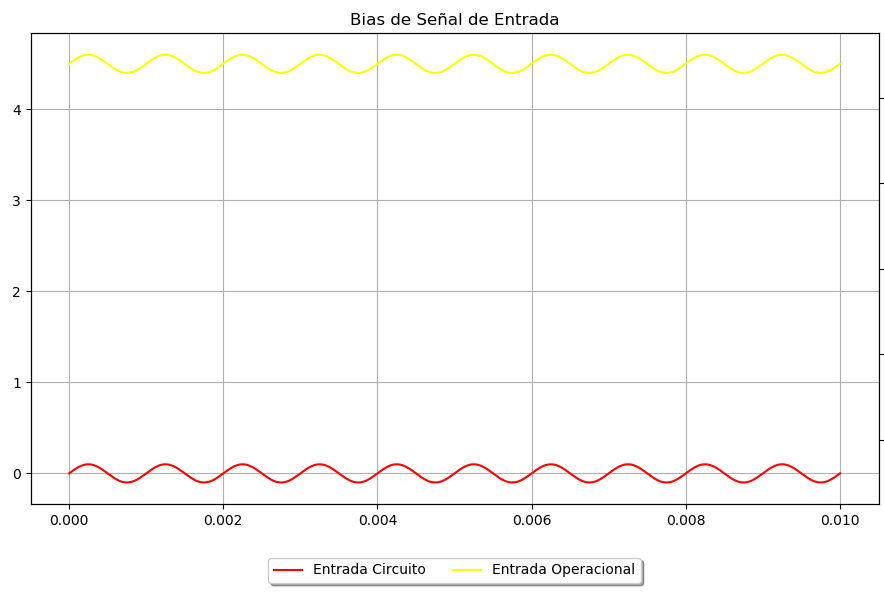
\includegraphics[width=1\textwidth, trim={0 0 0 0}, clip]{Ejercicio5/Imagenes/Circuito_base/Sim/circuito_base_tran_vi_viop.png}
	\caption{Análisis de la señal de entrada y señal de entrada al operacional.}
	\label{fig:sim_base}
\end{figure}
Se puede observar contrastando la señal de entrada con la señal que entra al opamp el correcto funcionamiento.
Luego, se analizó la señal de salida del opamp justo antes del capacitor de acople, en contraste a la señal de entrada al operacional.
\begin{figure}[H]
	\centering
	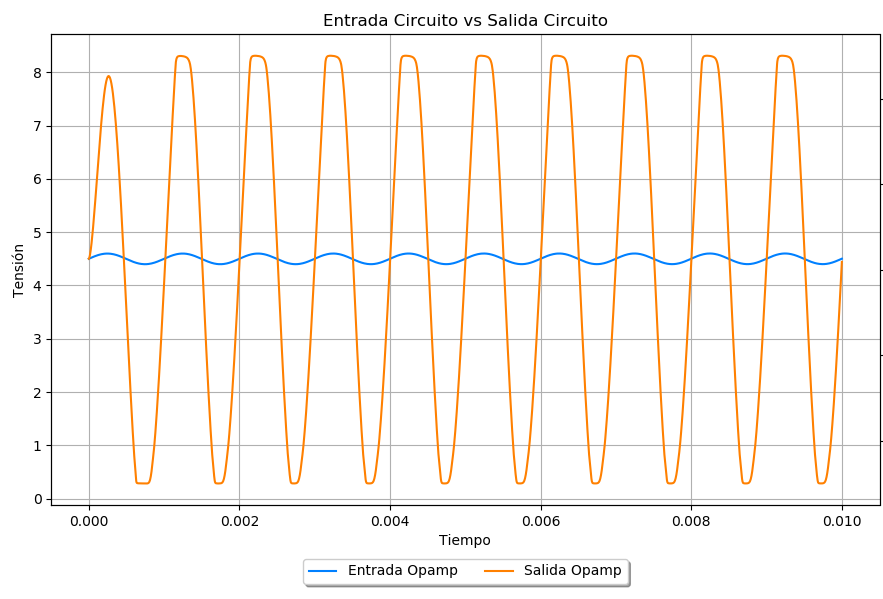
\includegraphics[width=1\textwidth, trim={0 0 0 0}, clip]{Ejercicio5/Imagenes/Circuito_base/Sim/circuito_base_tran_viop_voop.png}
	\caption{Análisis de la señal de entrada al operacional y señal de salida del operacional. }
	\label{fig:sim_base}
\end{figure}
Se puede observar como están presentes efectos distorsivos no lineales por culpa de la baja slew rate del operacional y por la saturación de este mismo, además de una gran amplificación.
Por último, se analizaron los efectos de la etapa de ecualización, contrastando la señal justo después del capacitor de acople a la salida del operacional, con la señal a la salida del circuito.

\begin{figure}[H]
	\centering
	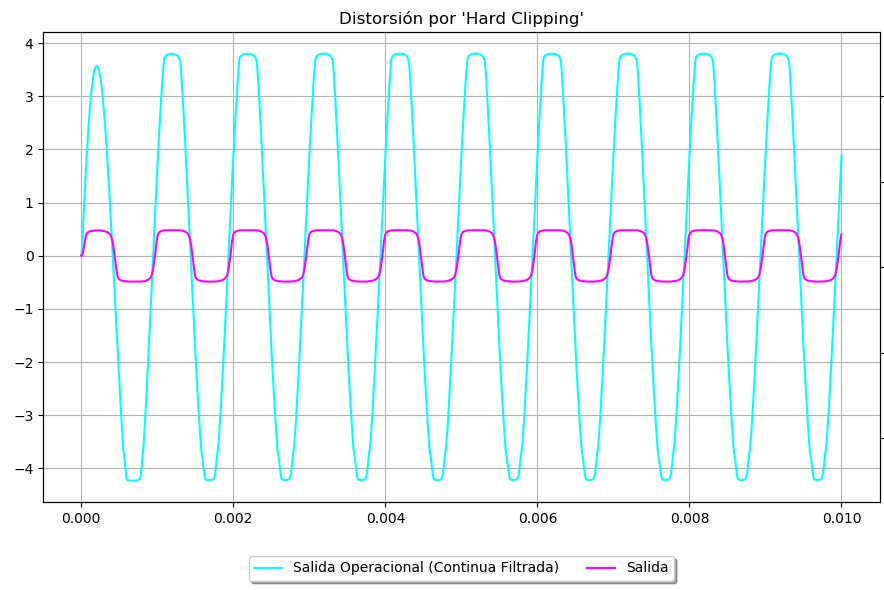
\includegraphics[width=1\textwidth, trim={0 0 0 0}, clip]{Ejercicio5/Imagenes/Circuito_base/Sim/circuito_base_tran_vclip_vo.png}
	\caption{Análisis de la señal de salida del operacional luego de filtrar la continua y señal de salida del circuito.}
	\label{fig:sim_base}
\end{figure}
Se puede contemplar como la señal es recortada por los diodos, generando una gran distorsión alineal.
Finalmente, para visualizar el funcionamiento total, se contrastaron las señales de entrada y salida del circuito.
\begin{figure}[H]
	\centering
	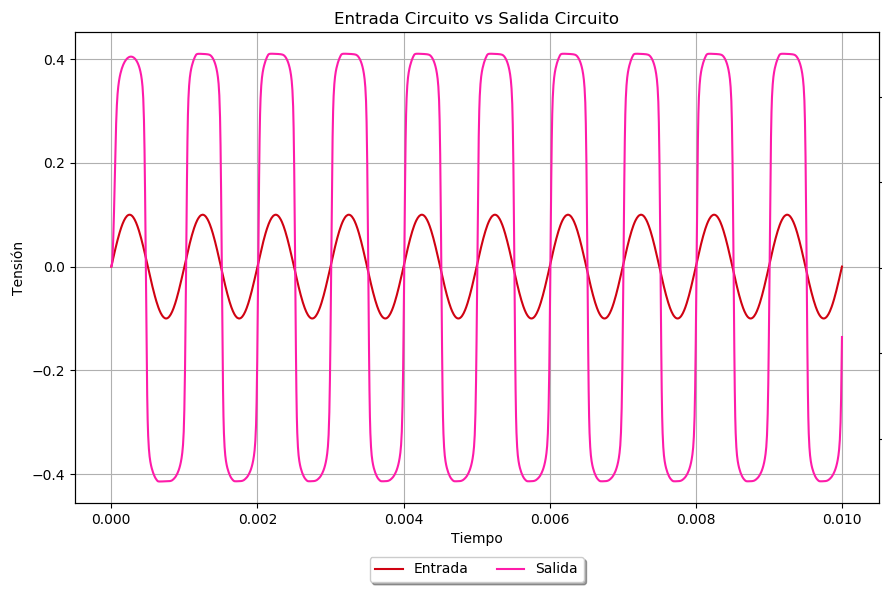
\includegraphics[width=1\textwidth, trim={0 0 0 0}, clip]{Ejercicio5/Imagenes/Circuito_base/Sim/circuito_base_tran_vi_vo.png}
	\caption{Análisis de la distorsión total en una señal de $100mV$ y $1kHz$.}
	\label{fig:sim_base}
\end{figure}
Contrastando ambas señales se puede observar el correcto funcionamiento calculado del circuito total.
\subsubsection{Análisis de Bode}
A continuación se simuló el gráfico de Bode de la transferencia de tensión entre la entrada y la salida del circuito.
\begin{figure}[H]
	\centering
	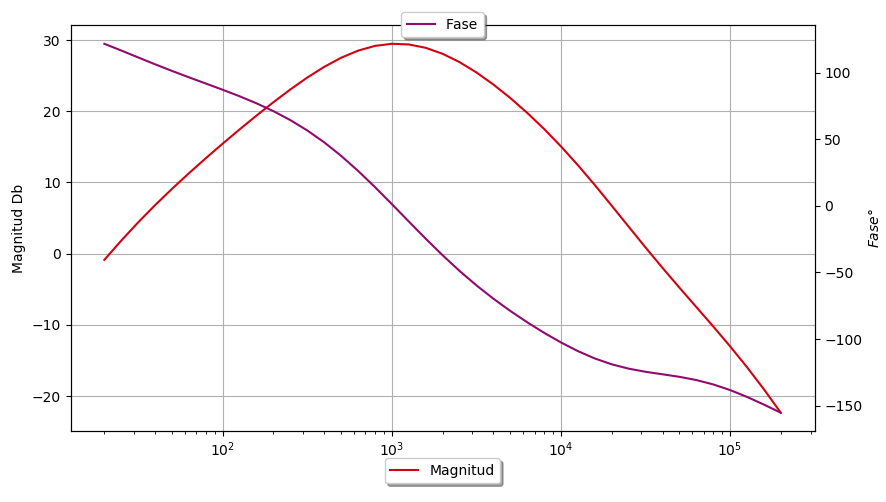
\includegraphics[width=1\textwidth, trim={0 0 0 0}, clip]{Ejercicio5/Imagenes/Circuito_base/Sim/circuito_base_bode.png}
	\caption{Gráfico de Bode para el circuito base.}
	\label{fig:sim_base}
\end{figure}

Se puede ver como hay un pico en la ganancia de $\approx 30dB$ alrededor de $1kHz$, mientras que los bajos y agudos son amplificados en menor medida. Se puede observar también como no habrán problemas de inestabilidad cuando el desfase introducido sea mayor de $180\deg$ ya que la atencuación ya será mayor a cero.

\subsubsection{Análisis de Fourier}

Se realizó un análisis de Fourier a la salida del circuito donde se pudo comprobar que hay un $29.76\%$ de distorsión armónica a la salida. La distorsión armónica es un parámetro para definir las señales de audio, en este caso nos está proporcionando una idea de los armónicos introducidos por la distorsión del circuito. Es calculado como el cociente entre el valor cuadrático medio de los armónicos de la señal empezando desde el segundo sobre el valor del primer armónico de la señal.
\begin{figure}[H]
	\centering
	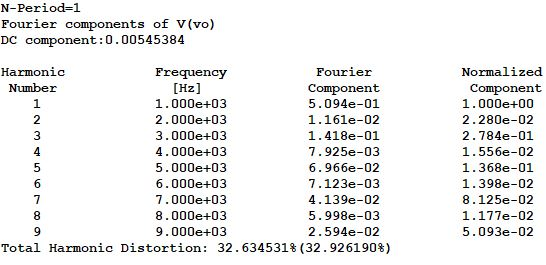
\includegraphics[width=1\textwidth, trim={0 0 0 0}, clip]{Ejercicio5/Imagenes/Circuito_base/Sim/sim_base_fourier.JPG}
	\caption{Análisis de las componentes de fourier y la distorsión armónica total.}
	\label{fig:sim_base_fourier}
\end{figure}
También se puede contemplar que los armónicos tienen un gran parecido con las componentes de fourier de una cuadrada, ya que los armónicos pares se ven más atenuados que los impares.

\subsection{Prototipo del Circuito Base}
Se realizó un prototipo del circuito base en un \textit{protoboard} con dos cambios: se suplantó la resistencia fija $R_4$ de un valor de $50k\Omega$ por un potenciómetro lineal de $250k\Omega$ y se agregó un diodo LED desde la alimentación de 9V hasta tierra, para indicar cuándo el circuito está alimentado. Luego, se quiso probar el circuito armado conectado con una guitarra a la entrada, y un amplificador de guitarra a la salida. Se utilizó una fuente de tensión continua no partida de 9V como alimentación. Por favor, referirse a los archivos 'ej5protobaseon.mp4' y 'ej5protobaseoff.mp4' para poder ver el resultado.
A lo largo de la prueba, se constataron dos puntos importantes:
\begin{itemize}
\item Se tuvo que utilizar el potenciómetro de $250k\Omega$ en el rango de aproximadamente $200k\Omega$ y $250k\Omega$ para obtener un nivel de saturación satisfactorio.
\item Los medios y agudos obtenían una buena distorsión, pero los bajos no lograban ser distorsionados del todo.
\end{itemize}
Estos dos puntos fueron gran causa de cambios en valores de resistores y capacitancias en el diseño propuesto.

\subsection{Diseño propuesto}

A continuación se presenta el diseño propuesto junto a un análisis de los componentes añadidos.

\subsubsection{Esquemático del diseño propuesto}

\vspace{1cm}
\hspace{-2cm}
\scalebox{0.7}{
\begin{circuitikz}

\draw

(0,0) node[spdt](bypass){}
	(bypass.in) ++ (-0.3,0) node[]{In}
	(bypass.out 2) to[short] ++ (0,-4)
		++ (0,-0.2) node[]{Bypass}
	(bypass.out 1) to[short] ++ (1,0)
		node[](n1){}
		
(n1) to[R=$1M\Omega$, *-] ++ (0,-3)
	node[ground]{}
	
(n1) to[C=$330nF$] ++ (3,0)
	node[](bias){}
	
(bias) to[R=$1M\Omega$, *-*] ++ (0, 3)
	node[](powbias){}
	
(powbias) to[short, -*] ++ (1,0)
	node[](aux4){}

(aux4) to[R=$10k\Omega$] ++ (0,-2)
	++ (0,0.3) node[ground]{}
	
(aux4) to[R=$10k\Omega$, -*] ++ (0,2)
	node[](powerrailmid){}
	
(aux4) to[C=$100pF$] ++ (1.5,0)
	node[ground]{}
	
(powerrailmid) to[short] ++ (-4,0)
	to[short] ++ (0,-3)
	to[short, -o] ++ (-1.3,0)
	++(-0.4,0) node[]{9V}

(powerrailmid) to[open] ++ (-3,0)
	to[C=$100\mu F$, *-] ++ (0,-2.5)
	node[ground]{}
	
(powerrailmid) to[short, -*] ++ (1.9,0)
	to[short] ++ (0,-4.8)
	++ (0.25, -0.22) node[](opamp_comp1){}
	
(powerrailmid) to[open] ++ (1.9,0)
	to[short] ++ (2, 0)
	to[R=$1k\Omega$] ++ (0, -2)
	to[led] ++ (0, -2)
	++ (0,0.2) node[ground]{}
	
(opamp_comp1) to[short] ++ (0, 2)
	to[C=$33pF$] ++ (1,0)
	to[short] ++ (0,-1)
	to[short] ++ (-0.5, 0)
	to[short] ++ (0,-1.25)

(bias) to[short] ++ (2,0)
	++ (1.15,-0.49) node[op amp, yscale=-1] (opamp){}
	++ (-0.1,0) node[]{LM308}
	
(opamp.-) to[short, -*] ++ (-0.3,0)
	node[](fbin){}
	to[short] ++ (-0.5,0)
	to[C=$1\mu F$] ++ (-1,0)
	to[short] ++ (-0.5,0)
	to[short] ++ (0,-2)
	to[R=$1k\Omega$] ++ (0,-2.235)
	++ (0, 0.2) node[ground]{}

(fbin) to[short] ++ (0,-2)
	node[](fbpar1_left){}
	to[pR=$250k\Omega$, *-*] ++ (3,0)
	node[](fbpar1_right){}
	to[short, -*] ++ (0,2.5)

(fbpar1_left) ++ (1.5,0.55) to[short] ++ (1,0)
	to[short] ++ (0,-0.55)
	
(fbpar1_left) to[open] ++ (0,0)
	to[C, l_=$560nF$, *-*] ++ (-2,0)
	
(opamp.up) node[ground]{}	

(opamp.out) to[short] ++ (0.3, 0)
	node[](fbout){}

(fbpar1_left) to[short] ++ (0, -1.5)
	node[](fbpar2_left){}
	to[switch] ++ (1,0)
	node[](aux2){}
	(aux2) to[short, *-] ++ (0,0.5)
		to[D] ++ (1,0)
	(aux2) to[short] ++ (0,-0.5)
		to[open] ++ (1,0)
		to[D] ++ (-1,0)
		to[open] ++ (1,0)
		to[short] ++ (0,1)
		to[open] ++ (0,-0.5)
		to[short, *-] ++ (1, 0)
		to[short] (fbpar1_right)

(fbout) to[C=$10\mu F$] ++ (1.5,0)
	to[R=$1k\Omega$] ++ (1.5,0)
	to[short, -*] ++ (0.5, 0)
	node[](hardclip){}

(hardclip) to[switch, -*] ++ (0,-1)
	node[](aux3){}
	(aux3) to[short] ++ (0.5,0)
		to[D] ++ (0, -1)
	(aux3) to[short] ++ (-0.5, 0)
		to[open] ++ (0,-1)
		to[D] ++ (0,1)
		to[open] ++ (0,-1)
		to[short] ++ (1,0)
		to[open, -*] ++ (-0.5, 0)
	(aux3) ++ (0,-1) to[short] ++ (0,-0.5) node[ground]{}
	
(hardclip) to[pR=$10k\Omega$] ++ (2.5,0)
	node[](aux6){}
	to[C=$10nF$] ++ (0,-2.745)
	++ (0,0.2) node[ground]{}

(hardclip) to[open] ++ (1.25, 1.05)
	to[short] ++ (0, 0.5)
	to[short] ++ (1.25,0)
	to[short] ++ (0, -1.55)
	
(aux6) to[short, *-] ++ (2,0)
	to[pR=$10k\Omega$] ++ (0,-2.5)
	node[ground]{}
	to[open] ++ (1.55,1.25)
	to[short] ++ (0.5,0)
	++ (0.3,0) node[]{Out}
	to[open] ++ (-0.5, 0)
	to[short, *-] ++ (0, -3)
	++ (0, -0.2) node[]{Bypass}
;

\end{circuitikz}

}

\vspace{1em}

\subsubsection{Análisis del Diseño Propuesto}

A continuación se presentan los cambios propuestos. No todos son cambios en el diseño sino también ajustes a valores de ciertos componentes luego de haber realizado simulaciones y haber prototipado el pedal con los valores calculados anteriormente.

\begin{itemize}
\item Se cambiaron los valores de las resistencias que generan el bias de la señal de entrada a $10k\Omega$, mientras que el punto medio del divisor resistivo se conecta a una nueva resistencia de $1M\Omega$. Esto permite elevar la impedancia de entrada del circuito con una sola resistencia de gran valor, en vez de proporcionar más ruido con dos resistencias de gran valor, si las resistencias del divisor fueran de $2M\Omega$. La nueva impedancia de entrada se calcularía aproximadamente como $$ 1M\Omega//\approx1M\Omega//10M\Omega $$ en el peor de los casos (con la mínima impedancia de entrada provista por el fabricante del operacional).
Además, se logra obtener una mucho mayor precisión a la hora de obtener $4,5V$, ya que la corriente que se escapa por el punto medio del divisor resistivo debe pasar por una resistencia de 100 veces el valor de la resistencia que tiene en paralelo.
\item Se agregó un capacitor en paralelo al punto medio del divisor resistivo para filtrar variaciones en el potencial que puedan hallarse. Se decidió que por más que sea un aumento en el costo final del producto el tener que agregar un componente más, sería a su vez un gran aumento en la calidad final, ya que cualquier pequeña variación en la tensión que se utiliza para levantar a la señal de entrada será amplificado con una muy grande ganancia al pasar por la etapa de amplificación, generando un gran ruido a la salida. La capacitancia fue calculada de tal manera que la frecuencia de corte del filtro pasa-altos que se forma con la resistencia de $10k\Omega$ se sitúe lo más alto posible. $$ f_c = \frac{1}{2\pi 10k\Omega 10pF} = 1.590MHz \approx 1,6MHz$$
\item Se cambió el valor del capacitor en el lazo de realimentación para favorecer la amplificación (también saturación y clipping) de los graves. El valor anterior se calculó con una frecuencia de corte de $500Hz$. Para el calculo del nuevo valor se posicionó el polo en los $100Hz$. $$C = \frac{1}{2\pi 100Hz 1k\Omega} = 1.591\mu F$$ por lo que se decidió utilizar un valor de $1uF + 560nF$ para ajustar a valores comerciales, posicionando finalmente el polo en una frecuencia de corte de  $$C = \frac{1}{2\pi 1.56\mu F 1k\Omega} = 102.02Hz$$.
\item Se agregó un diodo LED junto a su resistor para indicar cuándo está alimentado el circuito. También se agregaron dos llaves para activar o desactivar distintos tipos de distorsión. Esto añade mejor aspecto y una mayor funcionalidad al producto final y se justifica el precio de los componentes por esa razón.
\item Se decidió poner un potenciómetro en el lugar de la resistencia $R_4$ que anteriormente era de $50k\Omega$ para lograr tener una mayor funcionalidad y rangos de ganancia posibles en el circuito. Esto haría que la ganancia ideal de la etapa de amplificación esté aproximadamente entre 0 y 251. 
\item Se agregaron dos diodos con polaridad invertida en paralelo al potenciómetro en el lazo de realimentación. Este tipo de distorsión se la denomina \textit{soft clipping}, mientras que la distorsión provocada por los diodos a la salida del amplificador operacional se la denomina \textit{hard clipping}. Se decidió agregar este tipo de distorsión junto a una llave para agregar más funcionalidad al pedal. En el \textit{hard clipping} se recorta la señal que sale del operacional y proporciona una señal muy semejante a una cuadrada con gran componente de altas frecuencias, mientras que en el \textit{soft clipping}, como el recortado se realiza en el lazo de realimentación del operacional, se mezclan señales no recortadas con señales recortadas, produciendo una señal recortada mucho mas suave.
\textbf{pensar si no es mejor utilizar una llave inversora sin distorsion-soft-hard en vez de dos llaves, porque superponer soft con hard quiza no tenga mucho sentido.}
\item Se cambiaron los valores de las resistencias a la salida por dos resistores de $1k\Omega$. Esto se realizó ya que previamente se dejó un margen muy grande de seguridad al calcular los valores de los resistores y se decidió disminuir aún más la impedancia de salida. 
\item Se calculó nuevamente el filtro pasa-bajos de la salida. Antes se posicionó el polo en los $20kHz$, mientras que ahora estará situado en  aproximadamente $10kHz$. $$ f_c = \frac{1}{2\pi 2k\Omega 8.2nF} = 9.704kHz \approx 10kHz$$

\textbf{ver si poner el ultimo resistor un pote de 10k y el capacitor de 10nf, haria qeue el polo se corra de 1446,86 minimo a 15915,49 maximo. asi podria justificar porque baje tanto los resistores y en el minimo sigo estando dentro de una resistencia segura. sino otra es poner el primer resistor 100ohm y seguiria siendo 10 veces mas que la corriente maxima de continua que soporta el diodo 1n4148 y le meto un pote de 10k y un capa de 100n, entonces minimo seria 144,68hz y maximo 15,91khz}

\end{itemize}


\end{document}